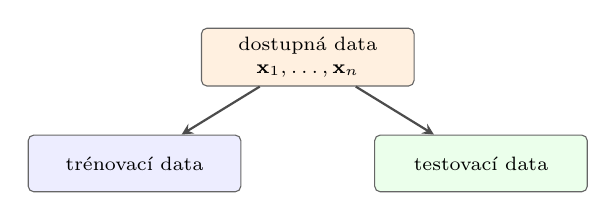
\begin{tikzpicture}[
    >=stealth,
    box/.style={
        draw=black!60,
        rounded corners=2pt,
        minimum width=2.7cm,
        minimum height=0.72cm,
        align=center,
        font=\scriptsize
    },
    arr/.style={->, thick, draw=black!70}
]
    \node[box, fill=orange!12] (data) at (0,1.35)
        {dostupná data\\$\mathbf{x}_1,\dots,\mathbf{x}_n$};

    \node[box, fill=blue!7] (train) at (-2.2,0)
        {trénovací data};

    \node[box, fill=green!8] (test) at (2.2,0)
        {testovací data};

    \draw[arr] (data) -- (train);
    \draw[arr] (data) -- (test);
\end{tikzpicture}
